\documentclass[a4paper,12pt]{article}
\usepackage[utf8]{inputenc}

\usepackage[utf8]{inputenc}
\usepackage[T2A]{fontenc}
\usepackage[english,russian]{babel}
\usepackage{amsthm}
\usepackage{amsmath}
\usepackage{amssymb}
\usepackage{tikz}
\usepackage{textcomp}
\usepackage{marvosym}
\usepackage{ esint }
\usepackage{mathtext}
\usepackage{siunitx} % Required for alignment
\usepackage{subfigure}
\usepackage{multirow}
\usepackage{rotating}
\usepackage{afterpage}
\usepackage[arrowdel]{physics}
\usepackage{booktabs}
\setlength{\topmargin}{-0.5in}
\setlength{\textheight}{9.1in}
\setlength{\oddsidemargin}{-0.4in}
\setlength{\evensidemargin}{-0.4in}
\setlength{\textwidth}{7in}
\setlength{\parindent}{0ex}
\setlength{\parskip}{1ex}
\newcommand{\ndiv}{\hspace{-4pt}\not|\hspace{2pt}}
\usepackage{graphicx}
\usepackage{float}
\usepackage{wrapfig}
\usepackage{pgfplots}
\usepackage{caption}
\pgfplotsset{compat=1.16}
\graphicspath{ {./images/} }
\usepackage{graphicx}
\RequirePackage{caption}
\DeclareCaptionLabelSeparator{defffis}{ — }
\captionsetup{justification=centering,labelsep=defffis}
\usepackage{caption} \captionsetup[table]{labelsep=endash,justification=justified,singlelinecheck=false,font=normalsize}
\usepackage{amsfonts,mathtools}
\newcommand{\eds}{\ensuremath{ \mathscr{E}}}

\title{Лабораторная работа № 3.4.5\\Петля гистерезиса(динамический метод)}
\author{Илья Прамский}
\date{Ноябрь 2023}

\begin{document}

\maketitle
\newpage

\paragraph*{Цель работы:} изучение петель гистерезиса ферромагнитных материалов с помощью осциллографа.
	
	\paragraph*{Оборудование:} автотрансформатор, понижающий трансформатор, амперметр и вольтметр (мультиметры), резистор, делитель напряжения, интегрирующая
	цепочка, электронный осциллогра, тороидальные образцы с двумя обмотками..
	
	\section{Теоретическое введение}
	
	\begin{wrapfigure}{l}{0.6\textwidth}
		\vspace{-20pt}
		\begin{center}			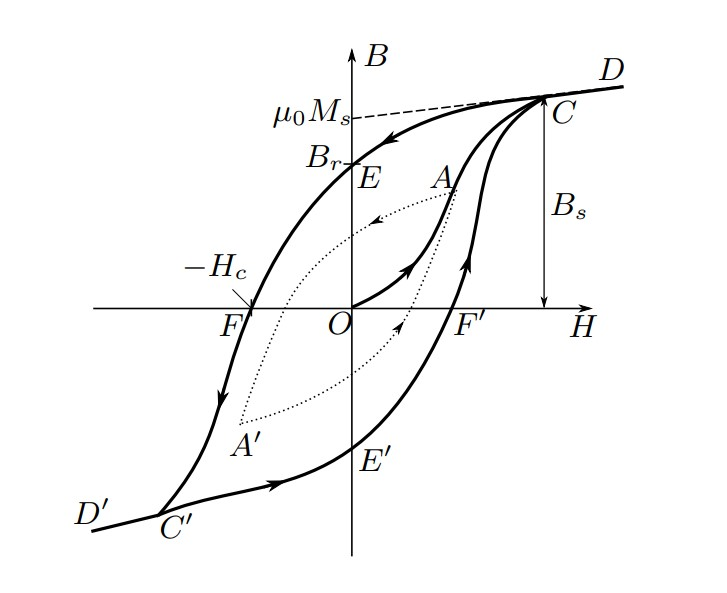
\includegraphics[width=0.7\linewidth]{gist3.jpg}
			\label{fig:sdfsafd}
		\end{center}
		\vspace{-10pt}
		\caption{Петля гистерезиса ферромагнетика}
	\end{wrapfigure}

	Магнитная индукция $\vec{B}$ и напряженность магнитного поля
	$\vec{H}$ в ферромагнитном материале неоднозначно связаны
	между собой: индукция зависит не только от напряженности, но
	и от предыстории образца. Связь между индукцией
	и напряженностью поля типичного ферромагнетика иллюстрирует рис. 1. Если
	к размагниченному образцу начинают прикладывать магнитное поле, то его намагничивание следует кривой $ OACD $, выходящей
	из начала
	координат. Эту кривую называют \textit{основной кривой намагничивания}.
	
	
	Индукция $\vec{B}$ в образце состоит из индукции, связанной с намагничивающим полем
	$\vec{B}$, и индукции, создаваемой самим намагниченным
	образцом.
	В системе СИ эта связь имеет вид
	
	$$\vec{B} = \mu_{0}(\vec{H}+\vec{M}),$$
	
	где $\vec{M}$- \textit{намагниченность} - магнитный момент единичного объема образца, а $\mu_{0}$ - магнитная постоянная.
	
	Намагнитим образец до насыщения - до точки D. Соответствующее
	значение индукции $B_{s}$ называют индукцией насыщения. При уменьшении поля $H$ до нуля зависимость $B(H)$ имеет вид кривой $DCE$, и при нулевом поле индукция имеет конечное ненулевое значение. Это остаточная индукция $B_{r}$ . Чтобы размагнитить образец, то есть перевести его в состояние
	$F$, необходимо приложить "обратное" магнитное
	поле $H_{c}$, которое называют коэрцитивной силой.
	
	Замкнутая кривая $DEFD'E'F'D$, возникающая при циклическом
	перемагничивании образца, намагниченного до насыщения, называется \textit{предельной петлей гистерезиса.}
	
	
	\subsection{Измерение магнитной индукции в образцах.}
	Магнитную индукцию удобно определять с помощью ЭДС, возникающей при изменении магнитного потока Ф в катушке, намотанной на образец:
	
	\[\mathcal{E} = -\dfrac{dФ}{dt}.\]
	
	Тогда отсюда и из формулы $Ф=BSN_{и}$ получаем:
		$$|B|=\dfrac{1}{SN_{и}}\int \mathcal{E} dt.$$
	Для интегрирования сигнала применяют интегрирующие схемы (рис. 2).
	
		\begin{wrapfigure}{l}{0.6\textwidth}
		\vspace{-20pt}
		\begin{center}
			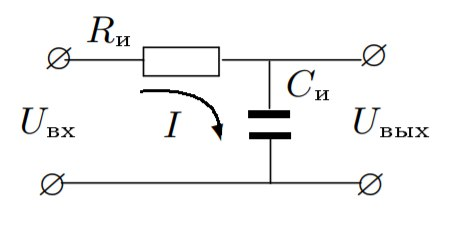
\includegraphics[width=0.7\linewidth]{gist2.jpg}
			\label{fig:sdfsafd}
		\end{center}
		\vspace{-10pt}
		\caption{Интегрирующая RC-цепь}
	\end{wrapfigure}
	
	Если выходной сигнал намного меньше входного ($U_{вых}\ll U_{вх},$) ток в цепи пропорционален входному напряжению: $I\simeq\dfrac{U_{вх}}{R}$, а напряжение на емкости С
	
	$$U_{вых}\simeq\dfrac{1}{RС}\int U_{вх}dt.$$
	
	Этот вывод тем ближе к истине, чем больше постоянная $\tau=RC$ превосходит характерное время процесса (например, его период). Для синусоидальных напряжений
	
	$$U_{вых}=\dfrac{U_{вх}}{RC\Omega},$$
	
	где $\Omega$ - частота сигнала.
	
	В итоге, обозначив параметры интегрирующей цепи через $R_{и}$ и $C_{и}$, получаем
	
	$$ |B|=\dfrac{1}{SN_{и}}\int U_{вх}dt=\dfrac{R_{и}С_{и}}{SN_{и}}U_{вых}.$$
	
	\section{Экспериментальная установка.}
	Схема экспериментальной установки показана на рис. 3.
	
	Действующее значение переменного тока в обмотке N0 измеряется амперметром А (мультиметром GDM). Последовательно с амперметром включено сопротивление $R_{0}$, напряжение с которого подается на вход X электронного осциллографа (ЭО). Это напряжение пропорционально току в обмотке $N_{0}$, а следовательно и напряженности H магнитного поля в образце.
	
	Для измерения магнитной индукции B с измерительной обмотки $N_{И}$ на вход интегрирующей RC -цепочки подается напряжение $U_{И}$ (UВХ), пропорциональное производной $\dot{B}$, а с выхода снимается напряжение $U_{C}$($U_{ВЫХ}$), пропорциональное
	величине B , и подается на вход Y осциллограа.
	Замкнутая кривая, возникающая на экране, воспроизводит в некотором масштабе (различном для осей X и Y ) петлю гистерезиса. Чтобы придать этой кривой количественный смысл, необходимо установить масштабы изображения, т.е. провести калибровку каналов X и Y ЭО. Для этого, во-первых, надо узнать, каким напряжениям (или токам) соответствуют амплитуды сигналов, видимых на экране, и во-вторых,  каким значениям B и H соответствуют эти напряжения
	(или токи).
	
	\begin{figure}[h!]
		\centering
		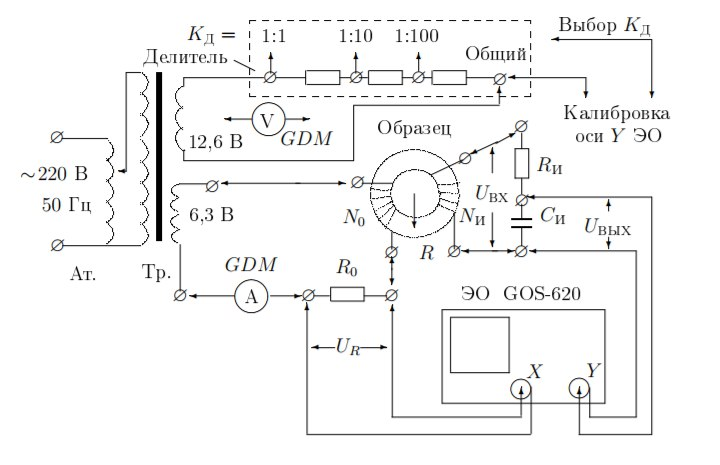
\includegraphics[width=\linewidth]{gist.jpg}
		\caption{Схема установки для исследования намагничивания образцов}
		\label{fig:Holl2}
	\end{figure}

\section{Ход работы}
Данные нашей установки: $R_0 = 0,3$ Ом, $R_\text{и} = 20$ кОм, $C_\text{и} = 20$ мкФ.

Теперь также выпишем данные каждой из обмоток:

Пермаллой(Fe-Ni НП50) $N_0 = 35$ витков, $N_\text{и} = 220$ витков, $S = 3,8$ cм$^2$, $2 \pi R = 24$ см;

Феррит 1000нн $N_0 = 35$ витков, $N_\text{и} = 400$ витков, $S = 3$ cм$^2$, $2 \pi R = 25$ см;

Кремнистое железо(Fe-Si) $N_0 = 35$ витков, $N_\text{и} = 350$ витков, $S = 1,2$ cм$^2$, $2 \pi R = 10$ см;

Теперь добьемся появления предельной петли гистерезиса и запишем чувствительность по оси x и по оси y у осциллографа.

Пермаллой $K_x = 20$мВ/дел, $K_y = 50$ мВ/дел;

Феррит $K_x = 20$мВ/дел, $K_y = 20$ мВ/дел;

Кремнистое железо $K_x = 50$мВ/дел, $K_y = 50$ мВ/дел;

Зная чувствительность для каждого из торойдов, найдем коэффициенты преобразования по осям электронного осциллографа в напряженность H и индукцию B.

\[H = \frac{I \cdot N_0}{2 \cdot \pi \cdot R}\]
Где $I= \frac{K_x}{R_0}$.
\[B = \frac{R_\text{и} \cdot C_\text{и}}{S \cdot N_\text{и}} \cdot U_\text{вых}\]
Где $U_\text{вых} = K_y$.

Получается

Пермаллой $H = 9,72$ Тл/дел, $B = 0,24$ Тл/дел;

Феррит $H = 9,3 $Тл/дел, $B = 0,06$ Тл/дел;

Кремнистое железо $ H = 58,3$Тл/дел, $B = 0,47$ Тл/дел.

Теперь, зная коэффициенты преобразования, найдем максимальные значения $B$ и $H$ у предельной петли для каждого из образцов. Полученные результаты занесём в таблицу.

Также найдем значения коэрцитивного поля $H_c$ и остаточной индукции $B_r$. Их тоже занесем в таблицу.

Дальше, проследив за движением крайней точки у гистерезиса, изобразим начальные кривые намагничивания $B(H)$ для каждого из образцов. По этим графикам оценим начальное и максимальное значения магнитной проницаемости $\mu_\text{диф}$. Результаты занесем в таблицу.

\begin{figure}[H]
	\begin{center}
    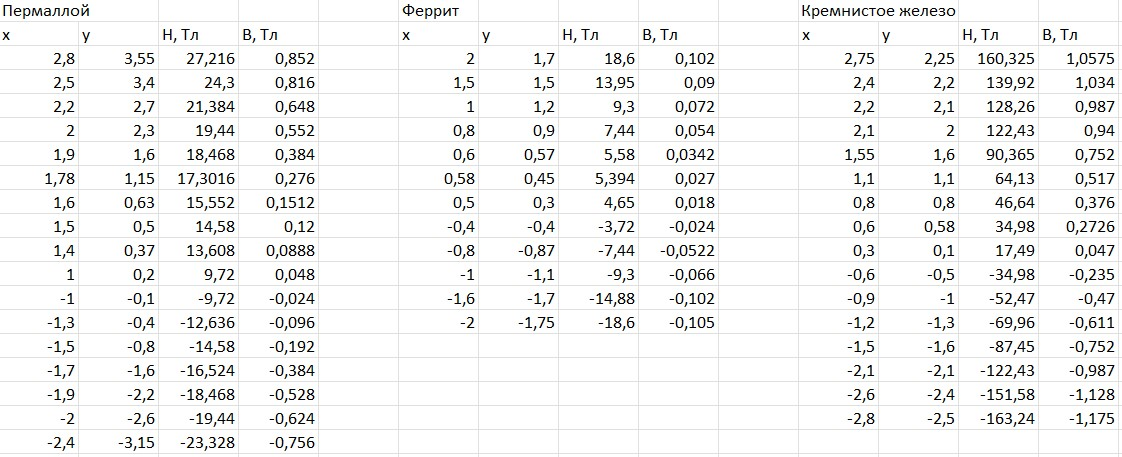
\includegraphics[width=0.75\textwidth]{tablizagist.jpg}
	\end{center}
\end{figure}

\begin{figure}[H]
	\begin{center}
    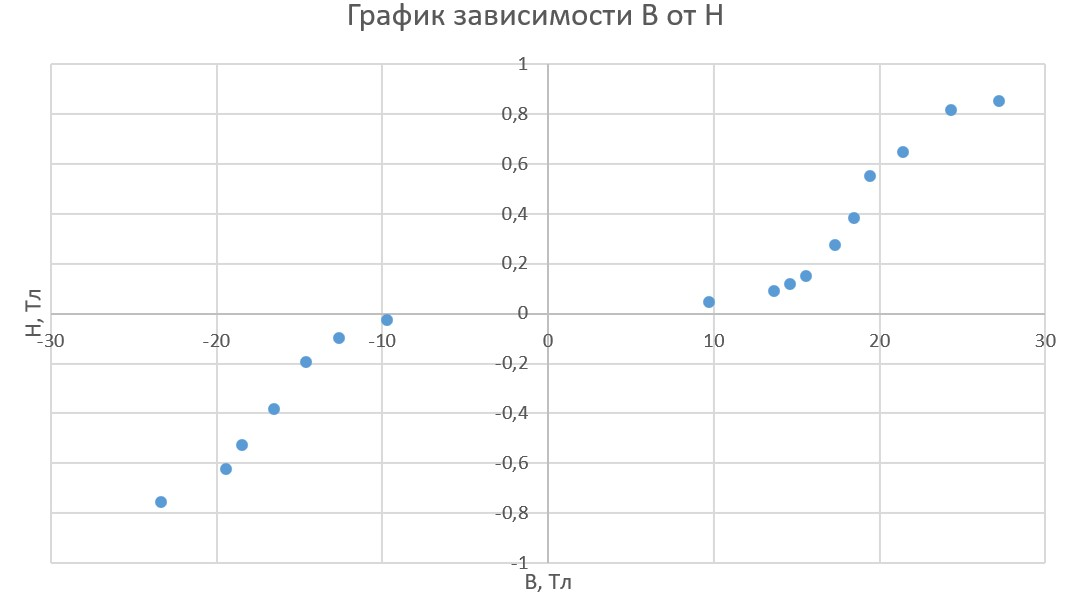
\includegraphics[width=0.5\textwidth]{graphikgist1.jpg}
    \caption{Пермаллой}
\label{fig:foobar}
	\end{center}
\end{figure}

\begin{figure}[H]
	\begin{center}
    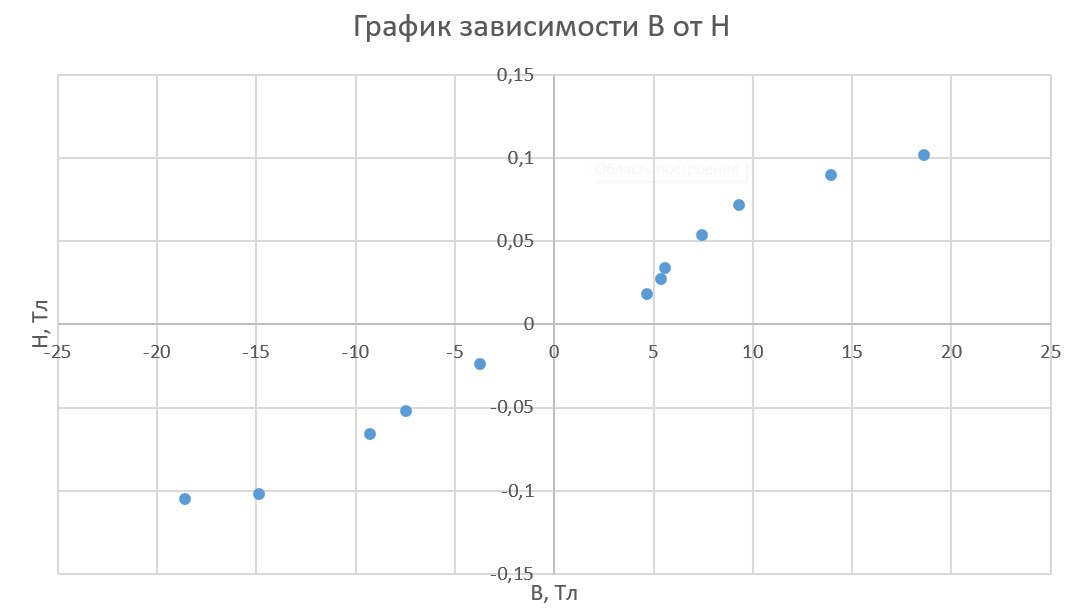
\includegraphics[width=0.5\textwidth]{graphikgist2.jpg}
    \caption{Феррит}
\label{fig:foobar}
	\end{center}
\end{figure}

\begin{figure}[H]
	\begin{center}
    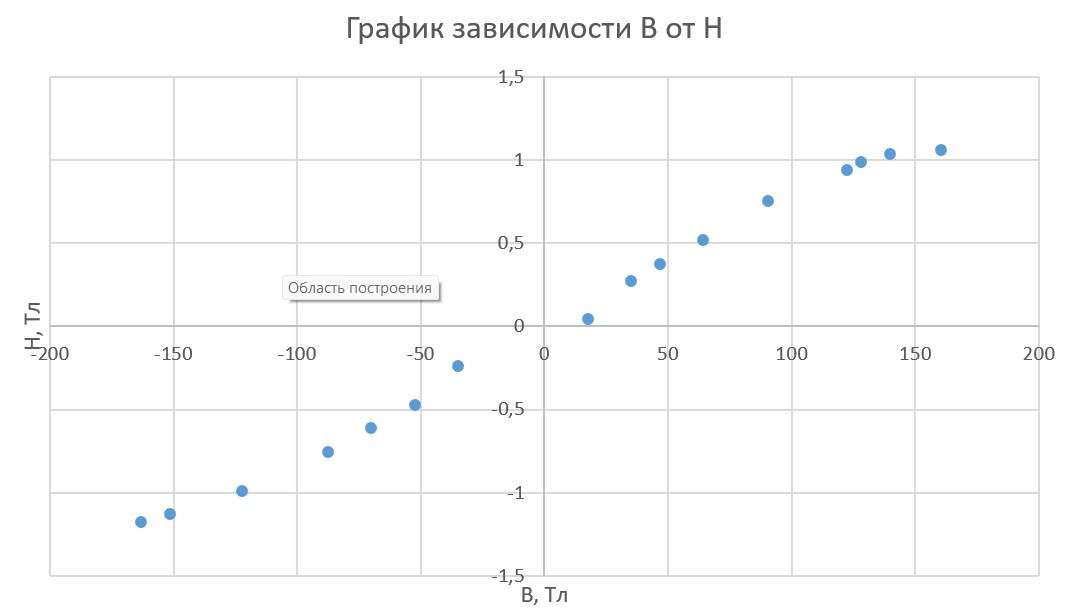
\includegraphics[width=0.5\textwidth]{graphikgist3.jpg}
    \caption{Кремнистое железо}
\label{fig:foobar}
	\end{center}
\end{figure}

\begin{figure}[H]
	\begin{center}
    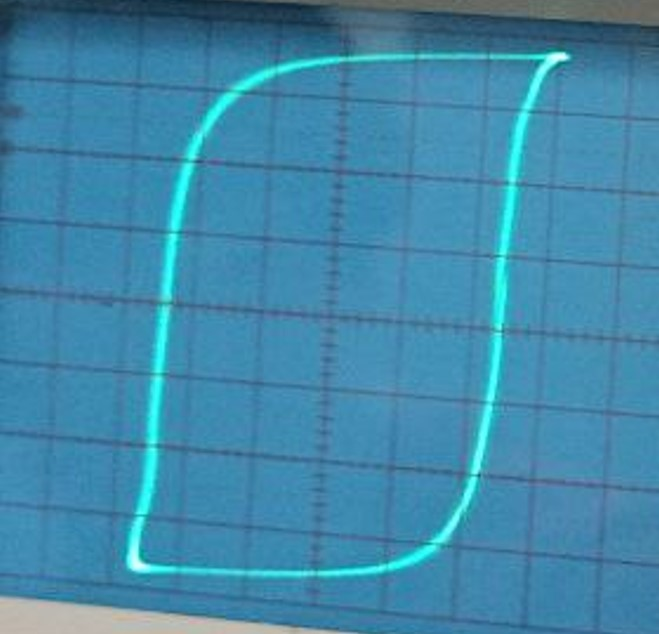
\includegraphics[width=0.5\textwidth]{photogist1.jpg}
    \caption{Пермаллой}
\label{fig:foobar}
	\end{center}
\end{figure}

\begin{figure}[H]
	\begin{center}
    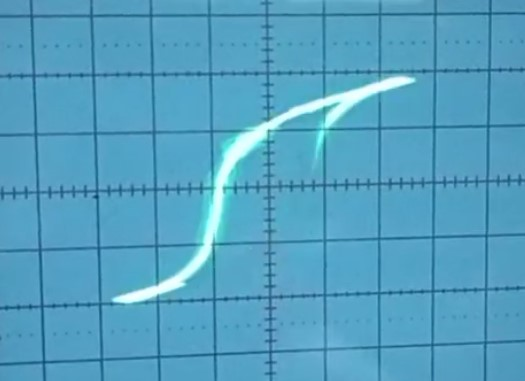
\includegraphics[width=0.5\textwidth]{photogist2.jpg}
    \caption{Феррит(график был нестабильным, из-за чего не удавалось получить на фото полный гистерезис)}
\label{fig:foobar}
	\end{center}
\end{figure}

\begin{figure}[H]
	\begin{center}
    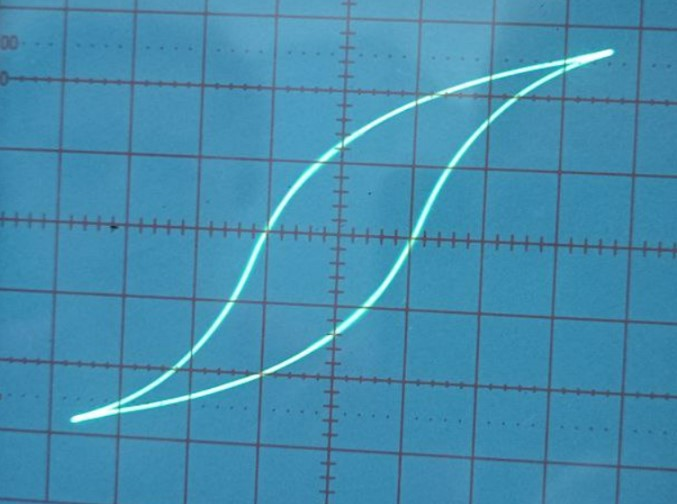
\includegraphics[width=0.5\textwidth]{photogist3.jpg}
    \caption{Кремнистое железо}
\label{fig:foobar}
	\end{center}
\end{figure}

Итоговая таблица
\begin{figure}[H]
	\begin{center}
    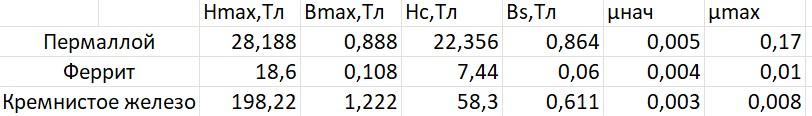
\includegraphics[width=0.5\textwidth]{itog.jpg}
\label{fig:foobar}
	\end{center}
\end{figure}

\section{Вывод}
В ходе работы были изучены петли гистерезиса различных торойдных образцов при помощи электронного осциллографа. При калибровке осциллографа также было получено, что его чувствительность достаточно точная(различие $10^{-3}$ порядка). С помощью изменения поданного питания, была получена начальная кривая намагничивания. При помощи её, а также предельной картины гистерезиса были оценены параметры торойдов, многие из которых порядка справочных($\mu$ сильно отличается от справочного значения. Связано это с тем, что при помощи отснятого процесса движения краевой точки, очень затруднительно фиксировать ее координаты каждый отрезок времени, из-за чего кривая намагничивания получилась неточной).
\end{document}

  
  	